\documentclass[1p]{elsarticle_modified}
%\bibliographystyle{elsarticle-num}

%\usepackage[colorlinks]{hyperref}
%\usepackage{abbrmath_seonhwa} %\Abb, \Ascr, \Acal ,\Abf, \Afrak
\usepackage{amsfonts}
\usepackage{amssymb}
\usepackage{amsmath}
\usepackage{amsthm}
\usepackage{scalefnt}
\usepackage{amsbsy}
\usepackage{kotex}
\usepackage{caption}
\usepackage{subfig}
\usepackage{color}
\usepackage{graphicx}
\usepackage{xcolor} %% white, black, red, green, blue, cyan, magenta, yellow
\usepackage{float}
\usepackage{setspace}
\usepackage{hyperref}

\usepackage{tikz}
\usetikzlibrary{arrows}

\usepackage{multirow}
\usepackage{array} % fixed length table
\usepackage{hhline}

%%%%%%%%%%%%%%%%%%%%%
\makeatletter
\renewcommand*\env@matrix[1][\arraystretch]{%
	\edef\arraystretch{#1}%
	\hskip -\arraycolsep
	\let\@ifnextchar\new@ifnextchar
	\array{*\c@MaxMatrixCols c}}
\makeatother %https://tex.stackexchange.com/questions/14071/how-can-i-increase-the-line-spacing-in-a-matrix
%%%%%%%%%%%%%%%

\usepackage[normalem]{ulem}

\newcommand{\msout}[1]{\ifmmode\text{\sout{\ensuremath{#1}}}\else\sout{#1}\fi}
%SOURCE: \msout is \stkout macro in https://tex.stackexchange.com/questions/20609/strikeout-in-math-mode

\newcommand{\cancel}[1]{
	\ifmmode
	{\color{red}\msout{#1}}
	\else
	{\color{red}\sout{#1}}
	\fi
}

\newcommand{\add}[1]{
	{\color{blue}\uwave{#1}}
}

\newcommand{\replace}[2]{
	\ifmmode
	{\color{red}\msout{#1}}{\color{blue}\uwave{#2}}
	\else
	{\color{red}\sout{#1}}{\color{blue}\uwave{#2}}
	\fi
}

\newcommand{\Sol}{\mathcal{S}} %segment
\newcommand{\D}{D} %diagram
\newcommand{\A}{\mathcal{A}} %arc


%%%%%%%%%%%%%%%%%%%%%%%%%%%%%5 test

\def\sl{\operatorname{\textup{SL}}(2,\Cbb)}
\def\psl{\operatorname{\textup{PSL}}(2,\Cbb)}
\def\quan{\mkern 1mu \triangleright \mkern 1mu}

\theoremstyle{definition}
\newtheorem{thm}{Theorem}[section]
\newtheorem{prop}[thm]{Proposition}
\newtheorem{lem}[thm]{Lemma}
\newtheorem{ques}[thm]{Question}
\newtheorem{cor}[thm]{Corollary}
\newtheorem{defn}[thm]{Definition}
\newtheorem{exam}[thm]{Example}
\newtheorem{rmk}[thm]{Remark}
\newtheorem{alg}[thm]{Algorithm}

\newcommand{\I}{\sqrt{-1}}
\begin{document}

%\begin{frontmatter}
%
%\title{Boundary parabolic representations of knots up to 8 crossings}
%
%%% Group authors per affiliation:
%\author{Yunhi Cho} 
%\address{Department of Mathematics, University of Seoul, Seoul, Korea}
%\ead{yhcho@uos.ac.kr}
%
%
%\author{Seonhwa Kim} %\fnref{s_kim}}
%\address{Center for Geometry and Physics, Institute for Basic Science, Pohang, 37673, Korea}
%\ead{ryeona17@ibs.re.kr}
%
%\author{Hyuk Kim}
%\address{Department of Mathematical Sciences, Seoul National University, Seoul 08826, Korea}
%\ead{hyukkim@snu.ac.kr}
%
%\author{Seokbeom Yoon}
%\address{Department of Mathematical Sciences, Seoul National University, Seoul, 08826,  Korea}
%\ead{sbyoon15@snu.ac.kr}
%
%\begin{abstract}
%We find all boundary parabolic representation of knots up to 8 crossings.
%
%\end{abstract}
%\begin{keyword}
%    \MSC[2010] 57M25 
%\end{keyword}
%
%\end{frontmatter}

%\linenumbers
%\tableofcontents
%
\newcommand\colored[1]{\textcolor{white}{\rule[-0.35ex]{0.8em}{1.4ex}}\kern-0.8em\color{red} #1}%
%\newcommand\colored[1]{\textcolor{white}{ #1}\kern-2.17ex	\textcolor{white}{ #1}\kern-1.81ex	\textcolor{white}{ #1}\kern-2.15ex\color{red}#1	}

{\Large $\underline{11n_{129}~(K11n_{129})}$}

\setlength{\tabcolsep}{10pt}
\renewcommand{\arraystretch}{1.6}
\vspace{1cm}\begin{tabular}{m{100pt}>{\centering\arraybackslash}m{274pt}}
\multirow{5}{120pt}{
	\centering
	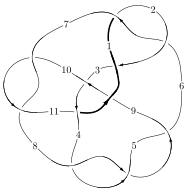
\includegraphics[width=112pt]{../../../GIT/diagram.site/Diagrams/png/745_11n_129.png}\\
\ \ \ A knot diagram\footnotemark}&
\allowdisplaybreaks
\textbf{Linearized knot diagam} \\
\cline{2-2}
 &
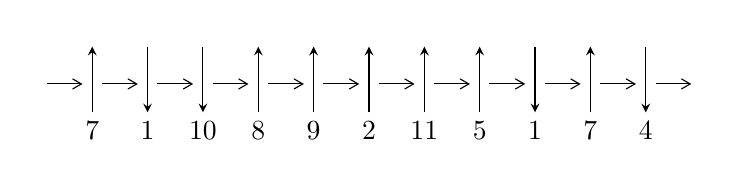
\begin{tikzpicture}[x=20pt, y=17pt]
	% nodes
	\node (C0) at (0, 0) {};
	\node (C1) at (1, 0) {};
	\node (C1U) at (1, +1) {};
	\node (C1D) at (1, -1) {7};

	\node (C2) at (2, 0) {};
	\node (C2U) at (2, +1) {};
	\node (C2D) at (2, -1) {1};

	\node (C3) at (3, 0) {};
	\node (C3U) at (3, +1) {};
	\node (C3D) at (3, -1) {10};

	\node (C4) at (4, 0) {};
	\node (C4U) at (4, +1) {};
	\node (C4D) at (4, -1) {8};

	\node (C5) at (5, 0) {};
	\node (C5U) at (5, +1) {};
	\node (C5D) at (5, -1) {9};

	\node (C6) at (6, 0) {};
	\node (C6U) at (6, +1) {};
	\node (C6D) at (6, -1) {2};

	\node (C7) at (7, 0) {};
	\node (C7U) at (7, +1) {};
	\node (C7D) at (7, -1) {11};

	\node (C8) at (8, 0) {};
	\node (C8U) at (8, +1) {};
	\node (C8D) at (8, -1) {5};

	\node (C9) at (9, 0) {};
	\node (C9U) at (9, +1) {};
	\node (C9D) at (9, -1) {1};

	\node (C10) at (10, 0) {};
	\node (C10U) at (10, +1) {};
	\node (C10D) at (10, -1) {7};

	\node (C11) at (11, 0) {};
	\node (C11U) at (11, +1) {};
	\node (C11D) at (11, -1) {4};
	\node (C12) at (12, 0) {};

	% arrows
	\draw[->,>={angle 60}]
	(C0) edge (C1) (C1) edge (C2) (C2) edge (C3) (C3) edge (C4) (C4) edge (C5) (C5) edge (C6) (C6) edge (C7) (C7) edge (C8) (C8) edge (C9) (C9) edge (C10) (C10) edge (C11) (C11) edge (C12) ;	\draw[->,>=stealth]
	(C1D) edge (C1U) (C2U) edge (C2D) (C3U) edge (C3D) (C4D) edge (C4U) (C5D) edge (C5U) (C6D) edge (C6U) (C7D) edge (C7U) (C8D) edge (C8U) (C9U) edge (C9D) (C10D) edge (C10U) (C11U) edge (C11D) ;
	\end{tikzpicture} \\
\hhline{~~} \\& 
\textbf{Solving Sequence} \\ \cline{2-2} 
 &
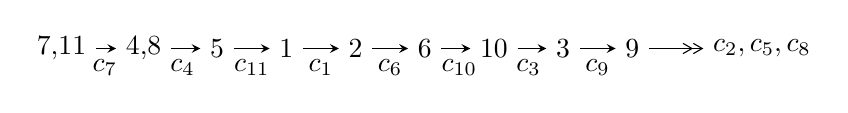
\begin{tikzpicture}[x=25pt, y=7pt]
	% node
	\node (A0) at (-1/8, 0) {7,11};
	\node (A1) at (17/16, 0) {4,8};
	\node (A2) at (17/8, 0) {5};
	\node (A3) at (25/8, 0) {1};
	\node (A4) at (33/8, 0) {2};
	\node (A5) at (41/8, 0) {6};
	\node (A6) at (49/8, 0) {10};
	\node (A7) at (57/8, 0) {3};
	\node (A8) at (65/8, 0) {9};
	\node (C1) at (1/2, -1) {$c_{7}$};
	\node (C2) at (13/8, -1) {$c_{4}$};
	\node (C3) at (21/8, -1) {$c_{11}$};
	\node (C4) at (29/8, -1) {$c_{1}$};
	\node (C5) at (37/8, -1) {$c_{6}$};
	\node (C6) at (45/8, -1) {$c_{10}$};
	\node (C7) at (53/8, -1) {$c_{3}$};
	\node (C8) at (61/8, -1) {$c_{9}$};
	\node (A9) at (10, 0) {$c_{2},c_{5},c_{8}$};

	% edge
	\draw[->,>=stealth]	
	(A0) edge (A1) (A1) edge (A2) (A2) edge (A3) (A3) edge (A4) (A4) edge (A5) (A5) edge (A6) (A6) edge (A7) (A7) edge (A8) ;
	\draw[->>,>={angle 60}]	
	(A8) edge (A9);
\end{tikzpicture} \\ 

\end{tabular} \\

\footnotetext{
The image of knot diagram is generated by the software ``\textbf{Draw programme}" developed by Andrew Bartholomew(\url{http://www.layer8.co.uk/maths/draw/index.htm\#Running-draw}), where we modified some parts for our purpose(\url{https://github.com/CATsTAILs/LinksPainter}).
}\phantom \\ \newline 
\centering \textbf{Ideals for irreducible components\footnotemark of $X_{\text{par}}$} 
 
\begin{align*}
I^u_{1}&=\langle 
-2.31440\times10^{35} u^{29}-4.29609\times10^{35} u^{28}+\cdots+1.17974\times10^{36} b-3.84219\times10^{36},\\
\phantom{I^u_{1}}&\phantom{= \langle  }1.35861\times10^{37} u^{29}+2.76955\times10^{37} u^{28}+\cdots+3.42123\times10^{37} a+4.28134\times10^{38},\\
\phantom{I^u_{1}}&\phantom{= \langle  }u^{30}+3 u^{29}+\cdots+120 u+29\rangle \\
I^u_{2}&=\langle 
u^6- u^5- u^2+b+2 u,\;- u^8+2 u^7-3 u^5+2 u^4- u^3+u^2+a+2 u-3,\\
\phantom{I^u_{2}}&\phantom{= \langle  }u^9-2 u^8- u^7+4 u^6- u^5- u^3-3 u^2+3 u+1\rangle \\
\\
\end{align*}
\raggedright * 2 irreducible components of $\dim_{\mathbb{C}}=0$, with total 39 representations.\\
\footnotetext{All coefficients of polynomials are rational numbers. But the coefficients are sometimes approximated in decimal forms when there is not enough margin.}
\newpage
\renewcommand{\arraystretch}{1}
\centering \section*{I. $I^u_{1}= \langle -2.31\times10^{35} u^{29}-4.30\times10^{35} u^{28}+\cdots+1.18\times10^{36} b-3.84\times10^{36},\;1.36\times10^{37} u^{29}+2.77\times10^{37} u^{28}+\cdots+3.42\times10^{37} a+4.28\times10^{38},\;u^{30}+3 u^{29}+\cdots+120 u+29 \rangle$}
\flushleft \textbf{(i) Arc colorings}\\
\begin{tabular}{m{7pt} m{180pt} m{7pt} m{180pt} }
\flushright $a_{7}=$&$\begin{pmatrix}1\\0\end{pmatrix}$ \\
\flushright $a_{11}=$&$\begin{pmatrix}0\\u\end{pmatrix}$ \\
\flushright $a_{4}=$&$\begin{pmatrix}-0.397110 u^{29}-0.809517 u^{28}+\cdots-36.6655 u-12.5140\\0.196180 u^{29}+0.364157 u^{28}+\cdots+15.5278 u+3.25682\end{pmatrix}$ \\
\flushright $a_{8}=$&$\begin{pmatrix}1\\- u^2\end{pmatrix}$ \\
\flushright $a_{5}=$&$\begin{pmatrix}-0.559813 u^{29}-1.18451 u^{28}+\cdots-55.4393 u-20.3298\\0.296144 u^{29}+0.567389 u^{28}+\cdots+24.3826 u+6.53699\end{pmatrix}$ \\
\flushright $a_{1}=$&$\begin{pmatrix}-0.434170 u^{29}-0.988757 u^{28}+\cdots-46.6121 u-16.4142\\0.0403473 u^{29}+0.114621 u^{28}+\cdots+7.11329 u+2.56728\end{pmatrix}$ \\
\flushright $a_{2}=$&$\begin{pmatrix}-0.393822 u^{29}-0.874135 u^{28}+\cdots-39.4988 u-13.8469\\0.0403473 u^{29}+0.114621 u^{28}+\cdots+7.11329 u+2.56728\end{pmatrix}$ \\
\flushright $a_{6}=$&$\begin{pmatrix}0.0125629 u^{29}-0.00130980 u^{28}+\cdots-1.04271 u+1.25453\\-0.247561 u^{29}-0.534045 u^{28}+\cdots-24.8763 u-7.72880\end{pmatrix}$ \\
\flushright $a_{10}=$&$\begin{pmatrix}- u\\u\end{pmatrix}$ \\
\flushright $a_{3}=$&$\begin{pmatrix}-0.550336 u^{29}-1.10515 u^{28}+\cdots-49.7304 u-17.0796\\0.349405 u^{29}+0.659790 u^{28}+\cdots+28.5927 u+7.82236\end{pmatrix}$ \\
\flushright $a_{9}=$&$\begin{pmatrix}0.330131 u^{29}+0.777311 u^{28}+\cdots+38.6348 u+14.8960\\-0.0389985 u^{29}-0.0361593 u^{28}+\cdots-0.253016 u-0.364324\end{pmatrix}$\\ \flushright $a_{9}=$&$\begin{pmatrix}0.330131 u^{29}+0.777311 u^{28}+\cdots+38.6348 u+14.8960\\-0.0389985 u^{29}-0.0361593 u^{28}+\cdots-0.253016 u-0.364324\end{pmatrix}$\\&\end{tabular}
\flushleft \textbf{(ii) Obstruction class $= -1$}\\~\\
\flushleft \textbf{(iii) Cusp Shapes $= -0.409930 u^{29}-0.752927 u^{28}+\cdots-34.5863 u+2.19818$}\\~\\
\newpage\renewcommand{\arraystretch}{1}
\flushleft \textbf{(iv) u-Polynomials at the component}\newline \\
\begin{tabular}{m{50pt}|m{274pt}}
Crossings & \hspace{64pt}u-Polynomials at each crossing \\
\hline $$\begin{aligned}c_{1},c_{6}\end{aligned}$$&$\begin{aligned}
&u^{30}+u^{29}+\cdots-10 u+1
\end{aligned}$\\
\hline $$\begin{aligned}c_{2}\end{aligned}$$&$\begin{aligned}
&u^{30}+37 u^{29}+\cdots+78 u+1
\end{aligned}$\\
\hline $$\begin{aligned}c_{3}\end{aligned}$$&$\begin{aligned}
&u^{30}+2 u^{29}+\cdots+423 u-121
\end{aligned}$\\
\hline $$\begin{aligned}c_{4},c_{5},c_{8}\end{aligned}$$&$\begin{aligned}
&u^{30}-2 u^{29}+\cdots+10 u-11
\end{aligned}$\\
\hline $$\begin{aligned}c_{7},c_{10}\end{aligned}$$&$\begin{aligned}
&u^{30}-3 u^{29}+\cdots-120 u+29
\end{aligned}$\\
\hline $$\begin{aligned}c_{9}\end{aligned}$$&$\begin{aligned}
&u^{30}-4 u^{29}+\cdots+1012 u-61
\end{aligned}$\\
\hline $$\begin{aligned}c_{11}\end{aligned}$$&$\begin{aligned}
&u^{30}-3 u^{29}+\cdots+80 u-7
\end{aligned}$\\
\hline
\end{tabular}\\~\\
\newpage\renewcommand{\arraystretch}{1}
\flushleft \textbf{(v) Riley Polynomials at the component}\newline \\
\begin{tabular}{m{50pt}|m{274pt}}
Crossings & \hspace{64pt}Riley Polynomials at each crossing \\
\hline $$\begin{aligned}c_{1},c_{6}\end{aligned}$$&$\begin{aligned}
&y^{30}+37 y^{29}+\cdots+78 y+1
\end{aligned}$\\
\hline $$\begin{aligned}c_{2}\end{aligned}$$&$\begin{aligned}
&y^{30}-79 y^{29}+\cdots+2922 y+1
\end{aligned}$\\
\hline $$\begin{aligned}c_{3}\end{aligned}$$&$\begin{aligned}
&y^{30}-36 y^{29}+\cdots-406651 y+14641
\end{aligned}$\\
\hline $$\begin{aligned}c_{4},c_{5},c_{8}\end{aligned}$$&$\begin{aligned}
&y^{30}-28 y^{29}+\cdots-122 y+121
\end{aligned}$\\
\hline $$\begin{aligned}c_{7},c_{10}\end{aligned}$$&$\begin{aligned}
&y^{30}-15 y^{29}+\cdots-7034 y+841
\end{aligned}$\\
\hline $$\begin{aligned}c_{9}\end{aligned}$$&$\begin{aligned}
&y^{30}-40 y^{29}+\cdots-182466 y+3721
\end{aligned}$\\
\hline $$\begin{aligned}c_{11}\end{aligned}$$&$\begin{aligned}
&y^{30}+15 y^{29}+\cdots-5378 y+49
\end{aligned}$\\
\hline
\end{tabular}\\~\\
\newpage\flushleft \textbf{(vi) Complex Volumes and Cusp Shapes}
$$\begin{array}{c|c|c}  
\text{Solutions to }I^u_{1}& \I (\text{vol} + \sqrt{-1}CS) & \text{Cusp shape}\\
 \hline 
\begin{aligned}
u &= -0.818507 + 0.418994 I \\
a &= \phantom{-}0.149226 - 1.014830 I \\
b &= \phantom{-}1.78901 + 1.43406 I\end{aligned}
 & -5.25125 + 0.68579 I & \phantom{-}5.61474 + 0.93865 I \\ \hline\begin{aligned}
u &= -0.818507 - 0.418994 I \\
a &= \phantom{-}0.149226 + 1.014830 I \\
b &= \phantom{-}1.78901 - 1.43406 I\end{aligned}
 & -5.25125 - 0.68579 I & \phantom{-}5.61474 - 0.93865 I \\ \hline\begin{aligned}
u &= \phantom{-}0.624245 + 0.671788 I \\
a &= \phantom{-}0.421688 + 1.150570 I \\
b &= -0.584922 - 0.354810 I\end{aligned}
 & \phantom{-}5.44904 + 2.23619 I & \phantom{-}4.08223 - 3.08847 I \\ \hline\begin{aligned}
u &= \phantom{-}0.624245 - 0.671788 I \\
a &= \phantom{-}0.421688 - 1.150570 I \\
b &= -0.584922 + 0.354810 I\end{aligned}
 & \phantom{-}5.44904 - 2.23619 I & \phantom{-}4.08223 + 3.08847 I \\ \hline\begin{aligned}
u &= -1.023250 + 0.383143 I \\
a &= -1.399580 + 0.049686 I \\
b &= -0.137063 - 0.842520 I\end{aligned}
 & -4.55029 - 3.91642 I & \phantom{-}4.57066 + 2.81955 I \\ \hline\begin{aligned}
u &= -1.023250 - 0.383143 I \\
a &= -1.399580 - 0.049686 I \\
b &= -0.137063 + 0.842520 I\end{aligned}
 & -4.55029 + 3.91642 I & \phantom{-}4.57066 - 2.81955 I \\ \hline\begin{aligned}
u &= -1.156040 + 0.034465 I \\
a &= \phantom{-}0.073453 - 0.680796 I \\
b &= -0.48025 + 1.49217 I\end{aligned}
 & \phantom{-}2.03013 + 0.06329 I & \phantom{-}5.83733 + 0.25546 I \\ \hline\begin{aligned}
u &= -1.156040 - 0.034465 I \\
a &= \phantom{-}0.073453 + 0.680796 I \\
b &= -0.48025 - 1.49217 I\end{aligned}
 & \phantom{-}2.03013 - 0.06329 I & \phantom{-}5.83733 - 0.25546 I \\ \hline\begin{aligned}
u &= \phantom{-}0.795313 + 0.244851 I \\
a &= \phantom{-}0.02386 + 1.42526 I \\
b &= \phantom{-}0.45732 - 1.49635 I\end{aligned}
 & \phantom{-}1.16010 + 2.70821 I & \phantom{-}1.48721 - 5.36654 I \\ \hline\begin{aligned}
u &= \phantom{-}0.795313 - 0.244851 I \\
a &= \phantom{-}0.02386 - 1.42526 I \\
b &= \phantom{-}0.45732 + 1.49635 I\end{aligned}
 & \phantom{-}1.16010 - 2.70821 I & \phantom{-}1.48721 + 5.36654 I\\
 \hline 
 \end{array}$$\newpage$$\begin{array}{c|c|c}  
\text{Solutions to }I^u_{1}& \I (\text{vol} + \sqrt{-1}CS) & \text{Cusp shape}\\
 \hline 
\begin{aligned}
u &= -0.873624 + 0.796874 I \\
a &= \phantom{-}0.740021 - 0.848178 I \\
b &= -0.138479 + 1.278340 I\end{aligned}
 & \phantom{-}4.61816 + 0.06790 I & \phantom{-}5.73031 - 0.16143 I \\ \hline\begin{aligned}
u &= -0.873624 - 0.796874 I \\
a &= \phantom{-}0.740021 + 0.848178 I \\
b &= -0.138479 - 1.278340 I\end{aligned}
 & \phantom{-}4.61816 - 0.06790 I & \phantom{-}5.73031 + 0.16143 I \\ \hline\begin{aligned}
u &= -0.796958\phantom{ +0.000000I} \\
a &= \phantom{-}1.72442\phantom{ +0.000000I} \\
b &= \phantom{-}0.0618987\phantom{ +0.000000I}\end{aligned}
 & \phantom{-}0.572803\phantom{ +0.000000I} & \phantom{-}10.1420\phantom{ +0.000000I} \\ \hline\begin{aligned}
u &= \phantom{-}0.718056 + 1.055960 I \\
a &= \phantom{-}0.821578 - 0.291189 I \\
b &= \phantom{-}0.111688 - 0.747195 I\end{aligned}
 & -9.10651 + 0.37265 I & -0.282021 + 0.198994 I \\ \hline\begin{aligned}
u &= \phantom{-}0.718056 - 1.055960 I \\
a &= \phantom{-}0.821578 + 0.291189 I \\
b &= \phantom{-}0.111688 + 0.747195 I\end{aligned}
 & -9.10651 - 0.37265 I & -0.282021 - 0.198994 I \\ \hline\begin{aligned}
u &= \phantom{-}1.115300 + 0.723201 I \\
a &= -0.038982 - 0.938537 I \\
b &= -1.15595 + 1.86596 I\end{aligned}
 & -7.65463 + 6.05562 I & \phantom{-}2.17136 - 4.65322 I \\ \hline\begin{aligned}
u &= \phantom{-}1.115300 - 0.723201 I \\
a &= -0.038982 + 0.938537 I \\
b &= -1.15595 - 1.86596 I\end{aligned}
 & -7.65463 - 6.05562 I & \phantom{-}2.17136 + 4.65322 I \\ \hline\begin{aligned}
u &= -1.167780 + 0.765588 I \\
a &= -0.272505 + 1.070770 I \\
b &= -0.35697 - 1.64614 I\end{aligned}
 & \phantom{-}5.69085 - 6.45106 I & \phantom{-}6.67961 + 5.50435 I \\ \hline\begin{aligned}
u &= -1.167780 - 0.765588 I \\
a &= -0.272505 - 1.070770 I \\
b &= -0.35697 + 1.64614 I\end{aligned}
 & \phantom{-}5.69085 + 6.45106 I & \phantom{-}6.67961 - 5.50435 I \\ \hline\begin{aligned}
u &= \phantom{-}1.37025 + 0.39698 I \\
a &= \phantom{-}0.223661 - 0.786242 I \\
b &= \phantom{-}0.280709 + 1.271790 I\end{aligned}
 & \phantom{-}8.63028 + 2.56200 I & \phantom{-}10.62309 + 0.27158 I\\
 \hline 
 \end{array}$$\newpage$$\begin{array}{c|c|c}  
\text{Solutions to }I^u_{1}& \I (\text{vol} + \sqrt{-1}CS) & \text{Cusp shape}\\
 \hline 
\begin{aligned}
u &= \phantom{-}1.37025 - 0.39698 I \\
a &= \phantom{-}0.223661 + 0.786242 I \\
b &= \phantom{-}0.280709 - 1.271790 I\end{aligned}
 & \phantom{-}8.63028 - 2.56200 I & \phantom{-}10.62309 - 0.27158 I \\ \hline\begin{aligned}
u &= \phantom{-}0.004317 + 0.547819 I \\
a &= -0.721264 + 1.206740 I \\
b &= \phantom{-}0.150599 + 0.025373 I\end{aligned}
 & -1.21990 - 1.07662 I & -2.59095 + 4.11373 I \\ \hline\begin{aligned}
u &= \phantom{-}0.004317 - 0.547819 I \\
a &= -0.721264 - 1.206740 I \\
b &= \phantom{-}0.150599 - 0.025373 I\end{aligned}
 & -1.21990 + 1.07662 I & -2.59095 - 4.11373 I \\ \hline\begin{aligned}
u &= -0.443842\phantom{ +0.000000I} \\
a &= -0.206304\phantom{ +0.000000I} \\
b &= -0.607008\phantom{ +0.000000I}\end{aligned}
 & \phantom{-}0.892044\phantom{ +0.000000I} & \phantom{-}12.1650\phantom{ +0.000000I} \\ \hline\begin{aligned}
u &= \phantom{-}1.55455 + 0.15333 I \\
a &= -0.406036 + 0.700408 I \\
b &= \phantom{-}0.17299 - 1.70175 I\end{aligned}
 & \phantom{-}3.98744 + 3.00009 I & \phantom{-}5.48464 - 3.04608 I \\ \hline\begin{aligned}
u &= \phantom{-}1.55455 - 0.15333 I \\
a &= -0.406036 - 0.700408 I \\
b &= \phantom{-}0.17299 + 1.70175 I\end{aligned}
 & \phantom{-}3.98744 - 3.00009 I & \phantom{-}5.48464 + 3.04608 I \\ \hline\begin{aligned}
u &= -1.48154 + 0.82940 I \\
a &= -0.017919 - 0.925838 I \\
b &= \phantom{-}0.78170 + 1.80867 I\end{aligned}
 & -1.77013 - 11.72040 I & \phantom{-}4.67233 + 5.69667 I \\ \hline\begin{aligned}
u &= -1.48154 - 0.82940 I \\
a &= -0.017919 + 0.925838 I \\
b &= \phantom{-}0.78170 - 1.80867 I\end{aligned}
 & -1.77013 + 11.72040 I & \phantom{-}4.67233 - 5.69667 I \\ \hline\begin{aligned}
u &= -0.54089 + 1.67235 I \\
a &= -0.545917 + 0.023732 I \\
b &= -0.117829 - 0.641723 I\end{aligned}
 & -5.21310 + 3.06517 I & \phantom{-}5.76591 - 3.12781 I \\ \hline\begin{aligned}
u &= -0.54089 - 1.67235 I \\
a &= -0.545917 - 0.023732 I \\
b &= -0.117829 + 0.641723 I\end{aligned}
 & -5.21310 - 3.06517 I & \phantom{-}5.76591 + 3.12781 I\\
 \hline 
 \end{array}$$\newpage\newpage\renewcommand{\arraystretch}{1}
\centering \section*{II. $I^u_{2}= \langle u^6- u^5- u^2+b+2 u,\;- u^8+2 u^7-3 u^5+2 u^4- u^3+u^2+a+2 u-3,\;u^9-2 u^8- u^7+4 u^6- u^5- u^3-3 u^2+3 u+1 \rangle$}
\flushleft \textbf{(i) Arc colorings}\\
\begin{tabular}{m{7pt} m{180pt} m{7pt} m{180pt} }
\flushright $a_{7}=$&$\begin{pmatrix}1\\0\end{pmatrix}$ \\
\flushright $a_{11}=$&$\begin{pmatrix}0\\u\end{pmatrix}$ \\
\flushright $a_{4}=$&$\begin{pmatrix}u^8-2 u^7+3 u^5-2 u^4+u^3- u^2-2 u+3\\- u^6+u^5+u^2-2 u\end{pmatrix}$ \\
\flushright $a_{8}=$&$\begin{pmatrix}1\\- u^2\end{pmatrix}$ \\
\flushright $a_{5}=$&$\begin{pmatrix}2 u^8-3 u^7-2 u^6+5 u^5-2 u^4+2 u^3-5 u+3\\- u^8+u^7+2 u^6- u^5-2 u^4- u^3+u^2+2 u+1\end{pmatrix}$ \\
\flushright $a_{1}=$&$\begin{pmatrix}u^8-2 u^7+3 u^5-2 u^4+u^3- u^2- u+3\\- u^6+u^5+u^4- u^3- u\end{pmatrix}$ \\
\flushright $a_{2}=$&$\begin{pmatrix}u^8-2 u^7- u^6+4 u^5- u^4- u^2-2 u+3\\- u^6+u^5+u^4- u^3- u\end{pmatrix}$ \\
\flushright $a_{6}=$&$\begin{pmatrix}- u^7+u^6+2 u^5-2 u^4- u^3+2\\u^5- u^4- u^3+u^2\end{pmatrix}$ \\
\flushright $a_{10}=$&$\begin{pmatrix}- u\\u\end{pmatrix}$ \\
\flushright $a_{3}=$&$\begin{pmatrix}u^8-2 u^7- u^6+4 u^5- u^4- u^2-3 u+3\\- u^4+u^3+u^2- u\end{pmatrix}$ \\
\flushright $a_{9}=$&$\begin{pmatrix}u^7- u^6-2 u^5+2 u^4+u^3+u^2- u-3\\- u^8+u^7+2 u^6-2 u^5- u^4+2 u\end{pmatrix}$\\ \flushright $a_{9}=$&$\begin{pmatrix}u^7- u^6-2 u^5+2 u^4+u^3+u^2- u-3\\- u^8+u^7+2 u^6-2 u^5- u^4+2 u\end{pmatrix}$\\&\end{tabular}
\flushleft \textbf{(ii) Obstruction class $= 1$}\\~\\
\flushleft \textbf{(iii) Cusp Shapes $= - u^8+u^7+2 u^6-4 u^5+u^2+4 u+1$}\\~\\
\newpage\renewcommand{\arraystretch}{1}
\flushleft \textbf{(iv) u-Polynomials at the component}\newline \\
\begin{tabular}{m{50pt}|m{274pt}}
Crossings & \hspace{64pt}u-Polynomials at each crossing \\
\hline $$\begin{aligned}c_{1}\end{aligned}$$&$\begin{aligned}
&u^9+5 u^7+9 u^5+u^4+8 u^3+u^2+3 u+1
\end{aligned}$\\
\hline $$\begin{aligned}c_{2}\end{aligned}$$&$\begin{aligned}
&u^9+10 u^8+43 u^7+106 u^6+167 u^5+173 u^4+116 u^3+45 u^2+7 u-1
\end{aligned}$\\
\hline $$\begin{aligned}c_{3}\end{aligned}$$&$\begin{aligned}
&u^9- u^8- u^7- u^6+3 u^4+3 u^3+4 u^2+2 u+1
\end{aligned}$\\
\hline $$\begin{aligned}c_{4},c_{5}\end{aligned}$$&$\begin{aligned}
&u^9- u^8-5 u^7+5 u^6+8 u^5-8 u^4-4 u^3+3 u^2+u+1
\end{aligned}$\\
\hline $$\begin{aligned}c_{6}\end{aligned}$$&$\begin{aligned}
&u^9+5 u^7+9 u^5- u^4+8 u^3- u^2+3 u-1
\end{aligned}$\\
\hline $$\begin{aligned}c_{7}\end{aligned}$$&$\begin{aligned}
&u^9-2 u^8- u^7+4 u^6- u^5- u^3-3 u^2+3 u+1
\end{aligned}$\\
\hline $$\begin{aligned}c_{8}\end{aligned}$$&$\begin{aligned}
&u^9+u^8-5 u^7-5 u^6+8 u^5+8 u^4-4 u^3-3 u^2+u-1
\end{aligned}$\\
\hline $$\begin{aligned}c_{9}\end{aligned}$$&$\begin{aligned}
&u^9-3 u^8+3 u^7-5 u^6+6 u^5+6 u^3-3 u^2-3 u-1
\end{aligned}$\\
\hline $$\begin{aligned}c_{10}\end{aligned}$$&$\begin{aligned}
&u^9+2 u^8- u^7-4 u^6- u^5- u^3+3 u^2+3 u-1
\end{aligned}$\\
\hline $$\begin{aligned}c_{11}\end{aligned}$$&$\begin{aligned}
&u^9-2 u^8+4 u^7-3 u^6+3 u^5- u^3+u^2- u-1
\end{aligned}$\\
\hline
\end{tabular}\\~\\
\newpage\renewcommand{\arraystretch}{1}
\flushleft \textbf{(v) Riley Polynomials at the component}\newline \\
\begin{tabular}{m{50pt}|m{274pt}}
Crossings & \hspace{64pt}Riley Polynomials at each crossing \\
\hline $$\begin{aligned}c_{1},c_{6}\end{aligned}$$&$\begin{aligned}
&y^9+10 y^8+43 y^7+106 y^6+167 y^5+173 y^4+116 y^3+45 y^2+7 y-1
\end{aligned}$\\
\hline $$\begin{aligned}c_{2}\end{aligned}$$&$\begin{aligned}
&y^9-14 y^8+\cdots+139 y-1
\end{aligned}$\\
\hline $$\begin{aligned}c_{3}\end{aligned}$$&$\begin{aligned}
&y^9-3 y^8- y^7+11 y^6+12 y^5-3 y^4-13 y^3-10 y^2-4 y-1
\end{aligned}$\\
\hline $$\begin{aligned}c_{4},c_{5},c_{8}\end{aligned}$$&$\begin{aligned}
&y^9-11 y^8+51 y^7-129 y^6+192 y^5-166 y^4+70 y^3- y^2-5 y-1
\end{aligned}$\\
\hline $$\begin{aligned}c_{7},c_{10}\end{aligned}$$&$\begin{aligned}
&y^9-6 y^8+15 y^7-16 y^6-3 y^5+24 y^4-13 y^3-15 y^2+15 y-1
\end{aligned}$\\
\hline $$\begin{aligned}c_{9}\end{aligned}$$&$\begin{aligned}
&y^9-3 y^8-9 y^7+23 y^6+48 y^5+18 y^4-10 y^3-45 y^2+3 y-1
\end{aligned}$\\
\hline $$\begin{aligned}c_{11}\end{aligned}$$&$\begin{aligned}
&y^9+4 y^8+10 y^7+13 y^6+3 y^5-12 y^4-11 y^3+y^2+3 y-1
\end{aligned}$\\
\hline
\end{tabular}\\~\\
\newpage\flushleft \textbf{(vi) Complex Volumes and Cusp Shapes}
$$\begin{array}{c|c|c}  
\text{Solutions to }I^u_{2}& \I (\text{vol} + \sqrt{-1}CS) & \text{Cusp shape}\\
 \hline 
\begin{aligned}
u &= -0.168914 + 0.950661 I \\
a &= \phantom{-}0.049336 - 0.609720 I \\
b &= -0.784185 - 0.982357 I\end{aligned}
 & -6.63247 + 1.79022 I & \phantom{-}1.84978 - 1.07531 I \\ \hline\begin{aligned}
u &= -0.168914 - 0.950661 I \\
a &= \phantom{-}0.049336 + 0.609720 I \\
b &= -0.784185 + 0.982357 I\end{aligned}
 & -6.63247 - 1.79022 I & \phantom{-}1.84978 + 1.07531 I \\ \hline\begin{aligned}
u &= -1.145600 + 0.103496 I \\
a &= \phantom{-}0.414158 - 0.863364 I \\
b &= -0.20585 + 1.62467 I\end{aligned}
 & \phantom{-}1.93998 + 1.74600 I & \phantom{-}4.48812 - 2.12055 I \\ \hline\begin{aligned}
u &= -1.145600 - 0.103496 I \\
a &= \phantom{-}0.414158 + 0.863364 I \\
b &= -0.20585 - 1.62467 I\end{aligned}
 & \phantom{-}1.93998 - 1.74600 I & \phantom{-}4.48812 + 2.12055 I \\ \hline\begin{aligned}
u &= \phantom{-}1.161230 + 0.594201 I \\
a &= -0.279042 - 0.783472 I \\
b &= \phantom{-}0.68024 + 1.36518 I\end{aligned}
 & \phantom{-}6.80275 + 0.69172 I & \phantom{-}8.39096 + 0.05325 I \\ \hline\begin{aligned}
u &= \phantom{-}1.161230 - 0.594201 I \\
a &= -0.279042 + 0.783472 I \\
b &= \phantom{-}0.68024 - 1.36518 I\end{aligned}
 & \phantom{-}6.80275 - 0.69172 I & \phantom{-}8.39096 - 0.05325 I \\ \hline\begin{aligned}
u &= \phantom{-}1.287590 + 0.340306 I \\
a &= -0.400111 + 1.033390 I \\
b &= \phantom{-}0.005983 - 1.355130 I\end{aligned}
 & \phantom{-}7.89851 + 3.55465 I & \phantom{-}6.26919 - 4.19762 I \\ \hline\begin{aligned}
u &= \phantom{-}1.287590 - 0.340306 I \\
a &= -0.400111 - 1.033390 I \\
b &= \phantom{-}0.005983 + 1.355130 I\end{aligned}
 & \phantom{-}7.89851 - 3.55465 I & \phantom{-}6.26919 + 4.19762 I \\ \hline\begin{aligned}
u &= -0.268618\phantom{ +0.000000I} \\
a &= \phantom{-}3.43132\phantom{ +0.000000I} \\
b &= \phantom{-}0.607619\phantom{ +0.000000I}\end{aligned}
 & -0.278310\phantom{ +0.000000I} & \phantom{-}0.00389950\phantom{ +0.000000I}\\
 \hline 
 \end{array}$$\newpage
\newpage\renewcommand{\arraystretch}{1}
\centering \section*{ III. u-Polynomials}
\begin{tabular}{m{50pt}|m{274pt}}
Crossings & \hspace{64pt}u-Polynomials at each crossing \\
\hline $$\begin{aligned}c_{1}\end{aligned}$$&$\begin{aligned}
&(u^9+5 u^7+\cdots+3 u+1)(u^{30}+u^{29}+\cdots-10 u+1)
\end{aligned}$\\
\hline $$\begin{aligned}c_{2}\end{aligned}$$&$\begin{aligned}
&(u^9+10 u^8+43 u^7+106 u^6+167 u^5+173 u^4+116 u^3+45 u^2+7 u-1)\\
&\cdot(u^{30}+37 u^{29}+\cdots+78 u+1)
\end{aligned}$\\
\hline $$\begin{aligned}c_{3}\end{aligned}$$&$\begin{aligned}
&(u^9- u^8- u^7- u^6+3 u^4+3 u^3+4 u^2+2 u+1)\\
&\cdot(u^{30}+2 u^{29}+\cdots+423 u-121)
\end{aligned}$\\
\hline $$\begin{aligned}c_{4},c_{5}\end{aligned}$$&$\begin{aligned}
&(u^9- u^8-5 u^7+5 u^6+8 u^5-8 u^4-4 u^3+3 u^2+u+1)\\
&\cdot(u^{30}-2 u^{29}+\cdots+10 u-11)
\end{aligned}$\\
\hline $$\begin{aligned}c_{6}\end{aligned}$$&$\begin{aligned}
&(u^9+5 u^7+\cdots+3 u-1)(u^{30}+u^{29}+\cdots-10 u+1)
\end{aligned}$\\
\hline $$\begin{aligned}c_{7}\end{aligned}$$&$\begin{aligned}
&(u^9-2 u^8- u^7+4 u^6- u^5- u^3-3 u^2+3 u+1)\\
&\cdot(u^{30}-3 u^{29}+\cdots-120 u+29)
\end{aligned}$\\
\hline $$\begin{aligned}c_{8}\end{aligned}$$&$\begin{aligned}
&(u^9+u^8-5 u^7-5 u^6+8 u^5+8 u^4-4 u^3-3 u^2+u-1)\\
&\cdot(u^{30}-2 u^{29}+\cdots+10 u-11)
\end{aligned}$\\
\hline $$\begin{aligned}c_{9}\end{aligned}$$&$\begin{aligned}
&(u^9-3 u^8+3 u^7-5 u^6+6 u^5+6 u^3-3 u^2-3 u-1)\\
&\cdot(u^{30}-4 u^{29}+\cdots+1012 u-61)
\end{aligned}$\\
\hline $$\begin{aligned}c_{10}\end{aligned}$$&$\begin{aligned}
&(u^9+2 u^8- u^7-4 u^6- u^5- u^3+3 u^2+3 u-1)\\
&\cdot(u^{30}-3 u^{29}+\cdots-120 u+29)
\end{aligned}$\\
\hline $$\begin{aligned}c_{11}\end{aligned}$$&$\begin{aligned}
&(u^9-2 u^8+4 u^7-3 u^6+3 u^5- u^3+u^2- u-1)\\
&\cdot(u^{30}-3 u^{29}+\cdots+80 u-7)
\end{aligned}$\\
\hline
\end{tabular}\newpage\renewcommand{\arraystretch}{1}
\centering \section*{ IV. Riley Polynomials}
\begin{tabular}{m{50pt}|m{274pt}}
Crossings & \hspace{64pt}Riley Polynomials at each crossing \\
\hline $$\begin{aligned}c_{1},c_{6}\end{aligned}$$&$\begin{aligned}
&(y^9+10 y^8+43 y^7+106 y^6+167 y^5+173 y^4+116 y^3+45 y^2+7 y-1)\\
&\cdot(y^{30}+37 y^{29}+\cdots+78 y+1)
\end{aligned}$\\
\hline $$\begin{aligned}c_{2}\end{aligned}$$&$\begin{aligned}
&(y^9-14 y^8+\cdots+139 y-1)(y^{30}-79 y^{29}+\cdots+2922 y+1)
\end{aligned}$\\
\hline $$\begin{aligned}c_{3}\end{aligned}$$&$\begin{aligned}
&(y^9-3 y^8- y^7+11 y^6+12 y^5-3 y^4-13 y^3-10 y^2-4 y-1)\\
&\cdot(y^{30}-36 y^{29}+\cdots-406651 y+14641)
\end{aligned}$\\
\hline $$\begin{aligned}c_{4},c_{5},c_{8}\end{aligned}$$&$\begin{aligned}
&(y^9-11 y^8+51 y^7-129 y^6+192 y^5-166 y^4+70 y^3- y^2-5 y-1)\\
&\cdot(y^{30}-28 y^{29}+\cdots-122 y+121)
\end{aligned}$\\
\hline $$\begin{aligned}c_{7},c_{10}\end{aligned}$$&$\begin{aligned}
&(y^9-6 y^8+15 y^7-16 y^6-3 y^5+24 y^4-13 y^3-15 y^2+15 y-1)\\
&\cdot(y^{30}-15 y^{29}+\cdots-7034 y+841)
\end{aligned}$\\
\hline $$\begin{aligned}c_{9}\end{aligned}$$&$\begin{aligned}
&(y^9-3 y^8-9 y^7+23 y^6+48 y^5+18 y^4-10 y^3-45 y^2+3 y-1)\\
&\cdot(y^{30}-40 y^{29}+\cdots-182466 y+3721)
\end{aligned}$\\
\hline $$\begin{aligned}c_{11}\end{aligned}$$&$\begin{aligned}
&(y^9+4 y^8+10 y^7+13 y^6+3 y^5-12 y^4-11 y^3+y^2+3 y-1)\\
&\cdot(y^{30}+15 y^{29}+\cdots-5378 y+49)
\end{aligned}$\\
\hline
\end{tabular}
\vskip 2pc
\end{document}